\documentclass[paper=a4, fontsize=11pt]{scrartcl}
\usepackage[T1]{fontenc}
\usepackage[utf8]{inputenc}
\usepackage{lmodern}
\usepackage{multirow}
\usepackage[table,xcdraw]{xcolor}
\usepackage[spanish]{babel}
\usepackage{cite}
\usepackage{amsmath,amsfonts,amsthm} % Math packages
\usepackage{graphics,graphicx, float} %para incluir imágenes y colocarlas
\usepackage[backref,colorlinks=true,linkcolor=black,urlcolor=blue,citecolor=blue]{hyperref} %Para crear enlaces en el pdf
\usepackage[noabbrev,spanish]{cleveref}
\usepackage{url}
\usepackage[shortlabels]{enumitem}
\usepackage{appendix}
\usepackage{eurosym}
\usepackage{epsfig}
\usepackage{caption}
\usepackage{subcaption}
\usepackage{cancel}

\usepackage{pgf}
\usepackage{tikz}
\usepackage{etoolbox}
\AtBeginEnvironment{tikzpicture}{\shorthandoff{>}\shorthandoff{<}}{}{}
\usetikzlibrary{arrows,automata,shapes}

\definecolor{mycolor}{RGB}{255,255,153}

\newcommand\Rcancel[1]{\renewcommand\CancelColor{\color{red}}\xcancel{#1}}
\newcommand\Blue[1]{ { \color{blue} #1} }


\renewcommand{\appendixname}{Anexo}
\renewcommand{\appendixtocname}{Anexo}
\renewcommand{\appendixpagename}{Anexo}

\numberwithin{figure}{section} % Number figures within sections (i.e. 1.1, 1.2, 2.1, 2.2 instead of 1, 2, 3, 4)
\numberwithin{table}{section} % Number tables within sections (i.e. 1.1, 1.2, 2.1, 2.2 instead of 1, 2, 3, 4)
\newcommand{\horrule}[1]{\rule{\linewidth}{#1}} % Create horizontal rule command with 1 argument of height

\title{
    \normalfont \normalsize
    \textsc{{\textbf{Modelos de Computación(2015-2016)}} \\ Grado en Ingeniería Informática \\ Universidad de Granada} \\ [25pt] % Your university, school and/or department name(s)
    \horrule{0.5pt} \\[0.4cm] % Thin top horizontal rule
    \huge Prácticas Modelos de Computación\\ % The assignment title
    \horrule{2pt} \\[0.5cm] % Thick bottom horizontal rule
}
\author{Antonio de la Vega Jiménez }


%*************************************************************


\begin{document}

\maketitle % Muestra el Título
\newpage %inserta un salto de página
\tableofcontents % para generar el índice de contenidos
\listoffigures
\newpage
\section{Práctica 1}
\textit{Explica con tus propias palabras que lenguaje genera la siguiente gramática: \newline
G=(V, T, P, S) donde V = {S, A, B} y T = {a, b} y las reglas de producción son:\vspace{2em}}

$ \hspace*{2.6cm}S\rightarrow aB \hspace{1cm} S\rightarrow bA  \hspace{1cm} A\rightarrow a\hspace{1cm}  A\rightarrow aS $\newline
$\hspace*{3cm} A\rightarrow bAA  \hspace{0.7cm} B\rightarrow b \hspace{1.3cm} B\rightarrow bS  \hspace{0.7cm} B\rightarrow aBB $\vspace{2em}

Esta gramática genera el lenguaje que esta formado por las cadenas de ``a'' y ``b'' que cumplen la condición de que el número de apariciones ``a'' es igual al número de apariciones ``b''. Como se pude ver en las producciones, al principio se puede añadir una ``a'' o una ``b'' , pero no se añaden solos, sino que se añaden junto a una variable, si se añade una ``a'' se añade junto a la variable ``B'' y si se añade una ``b'' se añade junto a la variable ``A''. La variable ``A'' y la variable ``B'' siempre acaban siendo sustituidas por una ``a'' y una ``b'' respectivamente, es decir se podría interpretar como que la variable  ``A''  significa añadir una  ``a''  y la variable  ``B''  añadir un  ``b'' , por ello al principio la ``a'' se añade junto a una ``B'' ( y  la ``b'' junto a una  ``A'') de forma que finalmente el número de ambos símbolos terminales será el mismo. Por ejemplo si empezamos con $S \rightarrow aB$ añadimos el símbolo terminal ``a'' a la cadena y la variable ``B'',  y como para quitar la ``B'' se acaba poniendo un ``b'', el número de símbolos terminales ``a'' y ``b'' esta equilibrado. En caso de querer añadir otra ``a'', hacemos uso de la producción $B\rightarrow aBB$, esta producción añade una``b'' de más , por lo que al usar las dos producciones anteriores quedaría la cadena $aaBB$ y como ``B'' siempre se acaba sustituyendo por ``b'' la cadena sigue cumpliendo la propiedad de que el número de apariciones de ``a'' es igual al número de apariciones de ``b''. Los símbolos ``a'' y ``b'' pueden ir apareciendo en cualquier orden ya que las producciones $B\rightarrow bS \  y\   A\rightarrow aS$ permiten cambiar entre un símbolo y otro manteniendo la propiedad de la cadena. En caso de que se comience por $S\rightarrow bA$ ocurre exactamente lo mismo.

\section{Práctica 2}
\textit{Determinar si G=({S, A, B}, {a, b ,c, d}, P, S) donde P es:}\vspace{1em} \newline
$ \hspace*{2.6cm}S\rightarrow AB \hspace{1cm} A\rightarrow Ab  \hspace{1cm} A\rightarrow a$ \newline
$\hspace*{2.6cm}  B\rightarrow cB \hspace{1cm}B\rightarrow d $\vspace{1em}\newline
\hspace*{2cm} \textit{genera un lenguaje de tipo 3 ( Regular ).} \newline

En primer lugar hay que mirar que lenguaje genera la gramática. Mirando las producciones se puede observar que la cadena tiene que empezar por $AB$ una vez tenemos eso a partir de ``A'' se pueden generar dos cosas , una ``a'' o una cadena de ``b'' que comienza con una ``a'' ya que la ``A'' solo se puede quitar añadiendo una ``a'', por lo tanto a partir de ``A'' se obtiene $\{ab^{i}\} :i \in \mathbb{N} $. A partir de la ``B'' se puede generar una ``d'' o una cadena de ``c'' con una una ``d'' al final. Por lo tanto el lenguaje generado es $\{ab^{i}c^{j}d\}: i,j \in \mathbb{N} $.  Para ver si es un lenguaje de tipo 3 tenemos que encontrar una gramática de tipo 3 que genere lo mismo que la anterior, es decir una gramatical que genere cadenas que comienzan por una ``a'' luego tengan todas las ``b'' que se quieran, después todas las ``c'' que se quiera y finalmente una ``d'' y que cumpla las condiciones ``$A \rightarrow uB\ o\ A\rightarrow u\ donde\ u \in T*\ y \ A,B \in V$'', por ejemplo nos vale la gramática $A\rightarrow aB,\ B\rightarrow bB,\ B\rightarrow C,\ C\rightarrow cC,\ C\rightarrow c$. Como en la jerarquía de Chomsky se dice que una gramática que cumple las condiciones anteriores genera un lenguaje de tipo 3 y la gramática que hemos creado cumple esas condiciones y genera el lenguaje $\{ab^{i}c^{j}d\}: i,j \in \mathbb{N} $, entonces el lenguaje es de tipo 3.

\section{Práctica 3}
\textit{Crear el autómata finito determinista que reconoce cadenas que comienzan con cualquier número de 1 y 0 (pudiendo no haber ninguno), luego contiene la subcadena \textbf{0110}, después tienen cualquier número de 1 y 0 (pudiendo no haber ninguno) , tras esto contiene la subcadena \textbf{1000} y finalmente tiene cualquier número de 0 y 1 (pudiendo no haber ninguno).  }
\newline

En primer lugar creamos el autómata finito no determinista mostrado en la figura \ref{fig1} que acepta las cadenas con la estructura que deseamos ( cadenas que empiezan con cualquier cosa, luego tiene la subcadena 0110 luego cualquier cosa , después la subcadena 1000 y finalmente cualquier cosa).
\begin{figure}[H]
\centering
\begin{tikzpicture}[->,>=stealth',shorten >=1pt,auto,node distance=2.8cm,semithick,initial text={Estado inicial}]
 \tikzstyle{every state}=[fill=mycolor]
\tikzstyle{every initial by arrow}=[text=red]
   \node[state,initial] (q0)   {$q_0$}; 
   \node[state] (q1) [ right of = q0] { $q_1$}; 
   \node[state] (q2) [right of = q1] {$q_2$}; 
   \node[state] (q3) [right of = q2] {$q_3$}; 
   \node[state] (q5) [below of = q0] {$q_5$}; 
   \node[state] (q6) [right of = q5] {$q_6$}; 
   \node[state] (q7) [right of = q6] {$q_7$}; 
   \node[state] (q8) [right of = q7] {$q_8$}; 
   \node[state,accepting](q9) [ right of =  q8] {$q_9$};
    \path[->] 
    (q0) edge  node {0} (q1)
      edge  [loop above] node {0,1} (q0)
    (q1) edge  node  {1} (q2)
    (q2) edge  node  {1} (q3)
    (q3) edge  node  {0} (q5)
    (q5) edge  node  {1} (q6)
      edge  [loop above] node {0,1} (q5)
    (q6) edge  node  {0} (q7)
    (q7) edge  node  {0} (q8)
    (q8) edge  node  {0} (q9)
    (q9) edge  [loop above] node {0,1} (q9);
\end{tikzpicture}
\caption{Autómata finito no determinista.} \label{fig1}
\end{figure}

\newpage
Una vez que tenemos el autómata finito no determinista ( figura \ref{fig1}) obtenemos el autómata finito determinista mostrado en la figura \ref{fig2} y ya tenemos un autómata finito determinista que reconoce cadenas con la estructura deseada.

\begin{figure}[H]
\centering
\begin{tikzpicture}[->,>=stealth',shorten >=1pt,auto,node distance=4cm,semithick,initial text={Estado inicial}]
 \tikzstyle{every state}=[fill=mycolor,ellipse]
 \tikzstyle{every initial by arrow}=[text=red]
 
   \node[state,initial] (q0)   {$\{q_0\}$}; 
   \node[state,node distance=3cm] (q01)   [ right of = q0] {$\{q_0 , q_1\}$};
   \node[state,node distance=3cm] (q02)   [ right of = q01] {$\{q_0 , q_2\}$};
   \node[state,node distance=2.5cm] (q03)   [ right of = q02] {$\{q_0 , q_3\}$};
   \node[state,node distance=2.5cm] (q015)   [ below of = q03] {$\{q_0 , q_1, q_5\}$};
   \node[state,node distance=2.5cm] (q0256) [ below of = q015] {$\{q_0, q_2, q_5, q_6\}$};
   \node[state] (q0356) [ left of = q0256] {$\{q_0 , q_3, q_5, q_6\}$};
   \node[state] (q056) [ left of = q0356] {$\{q_0 , q_5, q_6\}$};
   \node[state,node distance=2.5cm] (q0157) [below of = q0256] {$\{q_0 , q_1, q_5, q_7\}$};
   \node[state,node distance=2.5cm] (q0158) [ below of = q0157] {$\{q_0 , q_1, q_5, q_8\}$};
   \node[state,accepting,node distance=2.5cm] (q0159) [ below of = q0158] {$\{q_0 , q_1, q_5, q_9\}$};
   \node[state,accepting,node distance=5cm] (q02569) [ left of = q0159] {$\{q_0 , q_2, q_5, q_6, q_9\}$};
   \node[state,accepting,node distance=5cm] (q01579) [ left of = q02569] {$\{q_0 , q_1, q_5, q_7, q_9\}$};
   \node[state,accepting,node distance=2.5cm] (q01589) [ above of = q01579] {$\{q_0 , q_1, q_5, q_8, q_9\}$};
   \node[state,accepting,node distance=2.5cm] (q03569) [ below of = q02569] {$\{q_0 , q_3, q_5, q_6, q_9\}$};
   \node[state,accepting,node distance=2.5cm] (q0569) [ below of = q01579] {$\{q_0 , q_5, q_6, q_9\}$};

  \path[->] 
    (q0) edge  node {0} (q01)
    (q0) edge  [loop above] node {1} (q0)
    (q01) edge node {1} (q02)
    (q01) edge [loop above] node {0} (q01)
    (q02) edge node {1} (q03)
    (q02) edge [bend left] node {0} (q01)
    (q03) edge node {0} (q015)
    (q03) edge [bend left] node {1} (q0)
    (q015) edge [loop right] node {0} (q015)
    (q015) edge node {1} (q0256)
    (q0256) edge node {1} (q0356)
    (q0256) edge node {0} (q0157)
    (q0356) edge node {1} (q056)
    (q0356) edge node {0} (q0157)
    (q056) edge [loop below] node {1} (q056)
    (q056) edge [bend right] node {0} (q0157)
    (q0157) edge node {0} (q0158)
    (q0157) edge [bend left] node {1} (q0256)
    (q0158) edge [bend right=70] node {1} (q0256)
    (q0158) edge node {0} (q0159)
    (q0159) edge [loop right] node {0} (q0159)
    (q0159) edge node {1} (q02569)
    (q02569) edge node {0} (q01579)
    (q02569) edge node {1} (q03569)
    (q01579) edge [bend left] node {1} (q02569)
    (q01579) edge node {0} (q01589)
    (q01589) edge [bend left] node {1} (q02569)
    (q01589) edge [bend left] node {0} (q0159)
    (q03569) edge node {1} (q0569)
    (q03569) edge node {0} (q01579)
    (q0569) edge [loop below] node {1} (q0569)
    (q0569) edge node {0} (q01579);
    
\end{tikzpicture}
\caption{Autómata finito determinista.} \label{fig2}
\end{figure}

\section{Práctica 4}
\textit{Crear un fichero Lex con el código mostrado en el tema 2 y comprobar que funciona correctamente.}
\newline

Para esta practica he usado el fichero Lex del tema 2 con una pequeña modificación para que ademas de reconocer números  que usan  un ``.'' para los decimales , también reconozca a los que usan un ``,''. El fichero Lex es el mostrado en la figura \ref{lex}. Siguiendo el proceso mostrado en la figura \ref{prog} he comprobado que compila correctamente y además haciendo uso del archivo mostrado en la figura \ref{test} he comprobado que funciona adecuadamente.

\begin{figure}[H]
    \begin{center}
    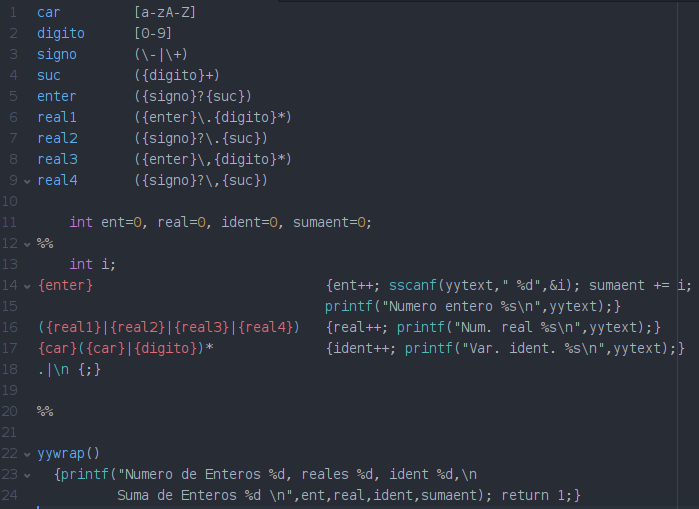
\includegraphics[width=1\textwidth]{Imagenes/lex}
        \caption{Fichero lex.}
        \label{lex}
    \end{center}
\end{figure}

\begin{figure}[H]
    \begin{center}
    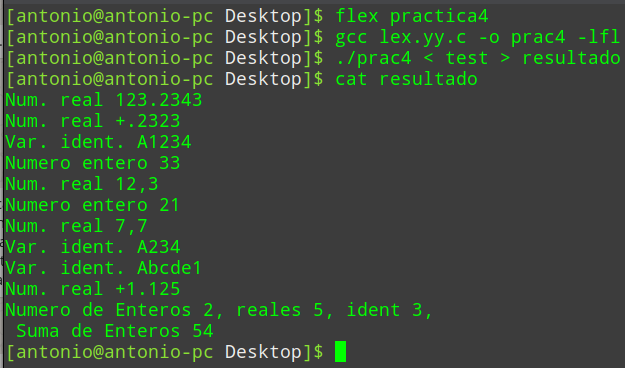
\includegraphics[width=0.7\textwidth]{Imagenes/prog}
        \caption{Proceso de compilación y ejecución del fichero lex.}
        \label{prog}
    \end{center}
\end{figure}

\begin{figure}[H]
    \begin{center}
    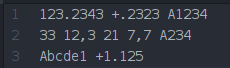
\includegraphics[width=0.5\textwidth]{Imagenes/test}
        \caption{Fichero para realizar la prueba.}
        \label{test}
    \end{center}
\end{figure}


\section{Práctica 5}
\textit{Dado el lenguaje $L = \{0u1\  /\ u \in \{0,1\}^{*}\}$ obtener la expresión regular, el autómata finito determinista y las gramáticas lineales por la izquierda y por la derecha.}
\newline

En primer lugar obtenemos la expresión regular que se corresponde con ese lenguaje, que seria la siguiente:\textbf{ \[ 0(0+1)^{*}1 \]}
Haciendo uso de la expresión regular podemos obtener el autómata finito no determinista con transiciones nulas mostrado en la figura \ref{fig3} que reconoce cadenas con esa estructura.
\begin{figure}[H]
\centering
\begin{tikzpicture}[->,>=stealth',shorten >=1pt,auto,node distance=2cm,semithick,initial text={Estado inicial}]
 \tikzstyle{every state}=[fill=mycolor]
 \tikzstyle{every initial by arrow}=[text=red]
 
    \node[state,initial] (q0)   {$q_0$}; 
   \node[state] (q2) [ right of = q0] { $q_2$}; 
   \node[state,node distance=2.5cm]  (q3) [above right  of = q2] {$q_3$}; 
   \node[state] (q4) [right of = q3] {$q_4$}; 
   \node[state,node distance=2.5cm] (q5) [below right of = q2] {$q_5$}; 
   \node[state] (q6) [right of = q5] {$q_6$}; 
   \node[state,node distance=2.5cm] (q7) [below right of = q4] {$q_7$}; 
   \node[state,accepting](q8) [ right of =  q7] {$q_8$};
   
     \path[->] 
    (q0) edge  node {0} (q2)
    (q2) edge  node {$\epsilon$ } (q3)
    (q2) edge  node {$\epsilon$ } (q5)
    (q3) edge  node {1} (q4)
    (q4) edge  node {$\epsilon$ } (q7)
    (q5) edge  node {0} (q6)
    (q6) edge  node {$\epsilon$ } (q7)
    (q2) edge [bend left=10]  node {$\epsilon$ } (q7)
    (q7) edge [bend left=10]  node {$\epsilon$ } (q2)
    (q7) edge  node {1} (q8);
\end{tikzpicture}
\caption{Autómata finito no determinista con transiciones nulas.} \label{fig3}
\end{figure}

A partir del autómata finito no determinista con transiciones nulas ( figura \ref{fig3}) obtenemos el autómata finito determinista de la figura \ref{fig4}.
\begin{figure}[H]
\centering
\begin{tikzpicture}[->,>=stealth',shorten >=1pt,auto,node distance=2cm,semithick,initial text={Estado inicial}]
 \tikzstyle{every state}=[fill=mycolor,ellipse]
 \tikzstyle{every initial by arrow}=[text=red]
 
   \node[state,initial] (q0)   {$\{q_0\}$}; 
   \node[state,node distance=4cm] (q2357) [ right of = q0] {$\{q_2,q_3,q_5,q_7\}$}; 
   \node[state,node distance=5cm]  (q23576) [right  of = q2357] {$\{q_2,q_3,q_5,q_7,q_6\}$}; 
   \node[state,accepting] (q235748) [below of = q23576] {$\{q_2,q_3,q_5,q_7,q_4,q_8\}$};
   \node[state] (vacio) [below of = q0] {$\emptyset$}; 
   
   \path[->] 
   (q0) edge node {0}(q2357)
   (q0) edge node {1} (vacio)
   (q2357) edge node {0} (q23576)
   (q2357) edge node {1} (q235748)
   (q23576) edge  [bend left=10]  node {1} (q235748)
   (q23576) edge [loop above]node {0} (q23576) 
   (vacio) edge [loop below] node {0,1} (vacio)
   (q235748)edge [bend left=10]  node {0} (q23576) 
   (q235748)edge [loop below] node {1} (q235748);
   
\end{tikzpicture}
\caption{Autómata finito determinista} \label{fig4}
\end{figure}

Para obtener la gramática lineal por la derecha hacemos uso del autómata anterior ( figura \ref{fig4} ) pero cambiamos los nombres de los nodos para que las producciones queden con nombres mas simples. El autómata resultante es el mostrado en la figura \ref{fig5}.
\begin{figure}[H]
\centering
\begin{tikzpicture}[->,>=stealth',shorten >=1pt,auto,node distance=2.5cm,semithick,initial text={Estado inicial}]
 \tikzstyle{every state}=[fill=mycolor,ellipse]
 \tikzstyle{every initial by arrow}=[text=red]
 
   \node[state,initial] (q0)  {$q_0$}; 
   \node[state] (q1) [ right of = q0] {$q_1$}; 
   \node[state] (q2) [right  of = q1] {$q_2$}; 
   \node[state,accepting] (q3) [below of = q2] {$q_3$};
   \node[state] (vacio) [below of = q0] {$q_4$}; 
   
   \path[->] 
   (q0) edge node {0}(q1)
   (q1) edge node {0} (q2)
   (q1) edge node {1} (q3)
   (q2) edge  [bend left=15]  node {1} (q3)
   (q2) edge [loop above]node {0} (q2) 
   (q3)edge [bend left=15]  node {0} (q2) 
   (q3)edge [loop below] node {1} (q3)
   (vacio) edge [loop below] node {0,1} (vacio)
   (q0) edge node {1} (vacio);
   
\end{tikzpicture}
\caption{Autómata \ref{fig4} simplificado.} \label{fig5}
\end{figure}
 Haciendo uso del autómata \ref{fig5} pasamos a obtener la gramática, que queda como se muestra a continuación ( el estado inicial es $q_0$ ):\vspace{0.5em} \newline
$ \hspace*{3cm}q_0\rightarrow 0q_1 \hspace{1cm} q_1\rightarrow 0q_2  \hspace{1cm} q_1\rightarrow 1q_3\hspace{1cm}  q_2\rightarrow 0q_2 $\newline
$\hspace*{3cm} q_2\rightarrow 1q_3  \hspace{1cm} q_3\rightarrow 0q_2 \hspace{1cm} q_3\rightarrow 1q_3  \hspace{1cm} q_3\rightarrow \varepsilon$
\newline$\hspace*{3cm} q_0\rightarrow 1q_4  \hspace{1cm} q_4\rightarrow 1q_4 \hspace{1cm} q_4\rightarrow 0q_4$  \vspace{2em}

Para obtener la gramática lineal por la izquierda, en primer lugar invertimos el autómata \ref{fig5} quedando como se muestra en la figura \ref{fig6}.
\begin{figure}[H]
\centering
\begin{tikzpicture}[->,>=stealth',shorten >=1pt,auto,node distance=2.5cm,semithick,initial text={Estado inicial}]
 \tikzstyle{every state}=[fill=mycolor,ellipse]
 \tikzstyle{every initial by arrow}=[text=red]
 
   \node[state,accepting] (q0)  {$q_0$}; 
   \node[state] (q1) [ right of = q0] {$q_1$}; 
   \node[state] (q2) [right  of = q1] {$q_2$}; 
   \node[state,initial] (q3) [below of = q2] {$q_3$};
   \node[state] (vacio) [below of = q0] {$q_4$}; 
   
   \path[->] 
   (q1) edge node {0}(q0)
   (q2) edge node {0} (q1)
   (q3) edge node {1} (q1)
   (q3) edge  [bend left=15]  node {1} (q2)
   (q2) edge [loop above]node {0} (q2) 
   (q2)edge [bend left=15]  node {0} (q3) 
   (q3)edge [loop below] node {1} (q3)
   (vacio) edge [loop below] node {0,1} (vacio)
   (vacio) edge node {1} (q0);;
   
\end{tikzpicture}
\caption{Autómata \ref{fig5} invertido.} \label{fig6}
\end{figure}


Como al invertir el autómata ha dejado de ser determinista hay que volverlo a convertir en determinista como se muestra a continuación:

\begin{figure}[H]
\centering
\begin{tikzpicture}[->,>=stealth',shorten >=1pt,auto,node distance=2.5cm,semithick,initial text={Estado inicial}]
 \tikzstyle{every state}=[fill=mycolor,ellipse]
 \tikzstyle{every initial by arrow}=[text=red]
    
   \node[state,initial] (q3) {$q_3$};
   \node[state] (q123) [right of = q3] {$\{q_1,q_2,q_3\}$};
   \node[state,accepting,node distance=3cm] (q1230) [below right of = q123] {$\{q_1,q_2,q_3,q_0\}$};
   \node[state] (vacio) [below of = q3] {$\emptyset$}; 
   
   \path[->] 
   (q3) edge node {1} (q123)
   (q3) edge node {0} (vacio)
   (q123) edge node {0} (q1230)
   (q123) edge [loop above] node {1} (q123)
   (q1230) edge [bend left] node {1} (q123)
   (q1230) edge [loop below] node {0} (q1230)
   (vacio) edge [loop below] node {0,1} (vacio);
   
\end{tikzpicture}
\caption{Autómata determinista obtenido del autómata \ref{fig6}} \label{fig7}
\end{figure}

Ahora simplificamos los nombres de los estados para que los nombres de las producciones sean mas sencillas:

\begin{figure}[H]
\centering
\begin{tikzpicture}[->,>=stealth',shorten >=1pt,auto,node distance=2.5cm,semithick,initial text={Estado inicial}]
 \tikzstyle{every state}=[fill=mycolor,ellipse]
 \tikzstyle{every initial by arrow}=[text=red]
    
   \node[state,initial] (q3) {$q_1$};
   \node[state] (q123) [right of = q3] {$q_2$};
   \node[state,accepting,node distance=3cm] (q1230) [below right of = q123] {$q_3$};
   \node[state] (vacio) [below of = q3] {$q_4$}; 
   
   \path[->] 
   (q3) edge node {1} (q123)
   (q3) edge node {0} (vacio)
   (q123) edge node {0} (q1230)
   (q123) edge [loop above] node {1} (q123)
   (q1230) edge [bend left] node {1} (q123)
   (q1230) edge [loop below] node {0} (q1230)
   (vacio) edge [loop below] node {0,1} (vacio);
   
\end{tikzpicture}
\caption{Autómata \ref{fig7} simplificado.} \label{fig8}
\end{figure}

\vspace{1em} A partir del autómata \ref{fig8} obtenemos la siguiente gramática ( el estado inicial es $q_1$ ): \vspace{0.5em} \newline

$\hspace*{1.8cm}q_1\rightarrow 0q_4 \hspace{1cm} q_1\rightarrow 1q_2  \hspace{1cm} q_2\rightarrow 1q_2\hspace{1cm}  q_2\rightarrow 0q_3 $\newline
$\hspace*{2.2cm} q_3\rightarrow 0q_3  \hspace{1cm} q_3\rightarrow 1q_2 \hspace{1cm} q_3\rightarrow \varepsilon  $\vspace{2em}

Por último invertimos la parte derecha de las producciones y obtenemos la gramática lineal por la izquierda mostrada a continuación  ( el estado inicial es $q_1$ ): \vspace{0.5em} \newline

$\hspace*{1.8cm}q_1\rightarrow q_40 \hspace{1cm} q_1\rightarrow q_21  \hspace{1cm} q_2\rightarrow q_21\hspace{1cm}  q_2\rightarrow q_30 $\newline
$\hspace*{2.2cm} q_3\rightarrow q_30  \hspace{1cm} q_3\rightarrow q_21 \hspace{1cm} q_3\rightarrow \varepsilon  $\vspace{2em}


\section{Práctica 6}
\textit{Proponer una gramática libre del contexto que contenga alguna producción nula y alguna producción unitaria. Eliminar las producciones nulas y unitarias y pasar a la forma normal de Chomsky.}
\newline
Para esta practica voy a usar la siguiente gramática:\vspace{0.5em} \newline
$ \hspace*{6cm}S\rightarrow A\  |\  BCa\  |\ aDcd $\newline
$ \hspace*{6cm}A\rightarrow aAb\ |\ c $\newline
$ \hspace*{6cm}B\rightarrow CD\  |\  Ad |\   \varepsilon $\newline
$ \hspace*{6cm}C\rightarrow Ca\  |\  Bb \ |\ c $\newline
$ \hspace*{6cm}D\rightarrow aDd\ |\ Dd\ |\ \varepsilon $\newline

En primer lugar buscamos y eliminamos las producciones nulas, tras esto la gramática queda de la siguiente forma:\vspace{0.5em} \newline
$ \hspace*{6cm}S\rightarrow A\  |\  BCa\  |\ aDcd \  |\Blue{\ Ca\ }  |\ \Blue{acd} $\newline
$ \hspace*{6cm}A\rightarrow aAb\ |\ c $\newline
$ \hspace*{6cm}B\rightarrow CD\  |\  Ad |\  \Rcancel{ \varepsilon} \  |\ \Blue{C}$\newline
$ \hspace*{6cm}C\rightarrow Ca\  |\  Bb \ |\ c \  |\ \Blue{b} $\newline
$ \hspace*{6cm}D\rightarrow aDd\ |\ Dd\ |\ \Rcancel{ \varepsilon} \  |\ \Blue{ad}\  |\ \Blue{d} $\newline

$\hspace*{6cm}H = \{B,D,S\}$\vspace{0.5em} 

El siguiente paso es eliminar las producciones unitarias, tras realizar esto, la gramática queda como se muestra a continuación:\vspace{0.5em} \newline

$ \hspace*{6cm}S\rightarrow \Rcancel{A}\  |\  BCa\  |\ aDcd \  |\ Ca\  |\ acd\  |\ \Blue{aAb}\  |\ \Blue{c} $\newline
$ \hspace*{6cm}A\rightarrow aAb\ |\ c $\newline
$ \hspace*{6cm}B\rightarrow CD\  |\  Ad  \ |\ \Rcancel{C} \  |\ \Blue{Ca}\  |\ \Blue{Bb}\  |\ \Blue{c}\  |\ \Blue{b} $\newline
$ \hspace*{6cm}C\rightarrow Ca\  |\  Bb \ |\ c \  |\ b $\newline
$ \hspace*{6cm}D\rightarrow aDd\ |\ Dd\ |\ ad\  |\ d $\newline

$\hspace*{6cm}H = \{B,D,S\}$\vspace{0.5em} 

Una vez que ya tenemos la gramática sin producciones nulas ni unitarias, la pasamos a la forma normal de Chomsky en la que todas las producciones tienen la forma $A\rightarrow BC \ o\ A\rightarrow a$.El primer paso para pasar a la forma normal de Chomsky es eliminar los símbolos terminales en las producciones que no sean $ A\rightarrow a$, tras hacer esto la gramática queda de la siguiente forma:\vspace{0.5em} \newline

$ \hspace*{2.2cm}X_a\rightarrow a $        $ \hspace*{1cm}S\rightarrow \  BCX_a\  |\ X_aDX_cX_d \  |\ CX_a\  |\ X_aX_cX_d\  |\ X_aAX_b\  |\ X_c $\newline
$ \hspace*{2.6cm}X_b\rightarrow b $        $ \hspace*{1cm}A\rightarrow X_aAX_b\ |\ X_c $\newline
$ \hspace*{2.6cm}X_c\rightarrow c  $        $ \hspace*{1cm}B\rightarrow CD\  |\  AX_d  \ \  |\ CX_a\  |\ BX_b\  |\ X_c\  |\ X_b $\newline
$ \hspace*{2.6cm}X_d\rightarrow d $        $ \hspace*{1cm}C\rightarrow CX_a\  |\  BX_b \ |\ X_c \  |\ X_b $\newline
                                                                              $ \hspace*{5cm}D\rightarrow X_aDX_d\ |\ DX_d\ |\ X_aX_d\  |\ X_d $\newline
\vspace{0.5em} 

Por último tenemos que quitar las producciones que tienen mas de dos variables a la derecha, tras hacer esto, nos queda:\vspace{0.5em} \newline

$ \hspace*{2.2cm}X_a\rightarrow a $        $ \hspace*{1cm}S\rightarrow \  \Rcancel{BCX_a\ }   |\Rcancel{\ X_aDX_cX_d \ } |\ CX_a\  |\Rcancel{\ X_aX_cX_d\ } |\Rcancel{\ X_aAX_b\ } |\ X_c $\newline
$ \hspace*{2.6cm}X_b\rightarrow b $        $ \hspace*{1cm}A\rightarrow \Rcancel{X_aAX_b\ } |\ X_c $\newline
$ \hspace*{2.6cm}X_c\rightarrow c  $        $ \hspace*{1cm}B\rightarrow CD\  |\  AX_d  \ \  |\ CX_a\  |\ BX_b\  |\ X_c\  |\ X_b $\newline
$ \hspace*{2.6cm}X_d\rightarrow d $        $ \hspace*{1cm}C\rightarrow CX_a\  |\  BX_b \ |\ X_c \  |\ X_b $\newline
                                                                              $ \hspace*{5cm}D\rightarrow \Rcancel{X_aDX_d\ }|\ DX_d\ |\ X_aX_d\  |\ X_d $\newline
                                                                              $ \hspace*{5cm}S\rightarrow \ \Blue{ BZ_1\   |\ X_aZ_2\   |\ X_aZ_4\  |\ X_aZ_5\  }$\newline
                                                                 \Blue{ $ \hspace*{5cm}A\rightarrow X_aZ_6 \hspace{1cm} D\rightarrow X_aZ_7  \hspace{0.9cm} Z_1\rightarrow CX_a\hspace{1cm}$ \newline
                                                                              $ \hspace*{5cm}Z_2\rightarrow DZ_3 \hspace{1cm} Z_3\rightarrow X_cX_d \hspace{0.8cm} Z_4\rightarrow X_cX_d\hspace{1cm}$ \newline
                                                                              $ \hspace*{5cm}Z_5\rightarrow AX_b\hspace{1cm} Z_6\rightarrow AX_b \hspace{1cm} Z_7\rightarrow DX_d\hspace{1cm}$ \newline}
\newpage                                                                      
Finalmente ordenando lo anterior, la gramática en forma normal de Chomsky es:\vspace{0.5em} \newline

$ \hspace*{2.2cm}X_a\rightarrow a $        $ \hspace*{1cm}S\rightarrow \  \ CX_a\  | \ X_c  \ | \ BZ_1\   |\ X_aZ_2\   |\ X_aZ_4\  |\ X_aZ_5\ $\newline
$ \hspace*{2.6cm}X_b\rightarrow b $        $ \hspace*{1cm}A\rightarrow \ X_c \  | \ X_aZ_6 $\newline
$ \hspace*{2.6cm}X_c\rightarrow c  $        $ \hspace*{1cm}B\rightarrow CD\  |\  AX_d  \ \  |\ CX_a\  |\ BX_b\  |\ X_c\  |\ X_b $\newline
$ \hspace*{2.6cm}X_d\rightarrow d $        $ \hspace*{1cm}C\rightarrow CX_a\  |\  BX_b \ |\ X_c \  |\ X_b $\newline
                                                                              $ \hspace*{5cm}D\rightarrow \ DX_d\ |\ X_aX_d\  |\ X_d \  | \ X_aZ_7$\newline
                                                                              $ \hspace*{5cm} Z_1\rightarrow CX_a\hspace{1cm}$ \newline
                                                                              $ \hspace*{5cm}Z_2\rightarrow DZ_3 \hspace{1cm} Z_3\rightarrow X_cX_d \hspace{0.8cm} Z_4\rightarrow X_cX_d\hspace{1cm}$ \newline
                                                                              $ \hspace*{5cm}Z_5\rightarrow AX_b\hspace{1cm} Z_6\rightarrow AX_b \hspace{1cm} Z_7\rightarrow DX_d\hspace{1cm}$ \newline
                                                                              
                                                                              
\section{Práctica 7}
\textit{Obtener una gramática libre del contexto que genere las palabras del lenguaje que reconoce un autómata con pila.}
\newline

Para realizar esta practica he elegido un autómata con pila que reconoce las palabras que contienen la misma cantidad de unos que de ceros:
\newline

$\hspace*{2.2cm}M=(\{q_1\},\{0,1\},\{R,X,Y\},\delta,q_1,R,\emptyset)$\newline

$\hspace*{2.2cm}\delta (q_1,0,R) = \{(q_1,XR)\}$                                                       $ \hspace*{1cm}\delta (q_1,0,X) = \{(q_1,XX)\}$\newline
$\hspace*{2.6cm}\delta (q_1,1,R) = \{(q_1,YR)\}$                                                        $ \hspace*{1cm}\delta (q_1,1,Y) = \{(q_1,YY)\}$\newline
$\hspace*{2.6cm}\delta (q_1,1,X) = \{(q_1,\varepsilon )\}$                                     $ \hspace*{1.4cm}\delta (q_1,0,Y) = \{(q_1,\varepsilon )\}$\newline
$\hspace*{2.6cm}\delta (q_1,\varepsilon ,R) = \{(q_1,\varepsilon )\}$\newline
\newline
A partir del autómata anterior obtenemos la siguiente gramática que genera las palabras que tiene el mismo número de unos que de ceros:
\newline

$ \hspace*{1.7cm} [q_1,R,q_1]\rightarrow 0[q_1,X,q_1][q_1,R,q_1] $      $ \hspace*{1.03cm} [q_1,X,q_1]\rightarrow 0[q_1,X,q_1][q_1,X,q_1] $   \newline
$ \hspace*{2.1cm} [q_1,R,q_1]\rightarrow 1[q_1,Y,q_1][q_1,R,q_1] $       $ \hspace*{1.1cm} [q_1,Y,q_1]\rightarrow 1[q_1,Y,q_1][q_1,Y,q_1] $   \newline
$ \hspace*{2.1cm} [q_1,X,q_1]\rightarrow 1 $                                             $ \hspace*{4.1cm} [q_1,Y,q_1]\rightarrow 0$   \newline
$ \hspace*{2.1cm} [q_1,R,q_1]\rightarrow \varepsilon  $   \newline




%*************************************************************



\end{document}
